% !TEX TS-program = XeLaTeX
% Commands for running this example:
% 	 xelatex Xindy_Make_Glossaries
%      xindy -L persian -C utf8 -I xindy -M Xindy_Make_Glossaries.xdy -t Xindy_Make_Glossaries.glg -o Xindy_Make_Glossaries.gls Xindy_Make_Glossaries.glo
% 	 xelatex Xindy_Make_Glossaries
% End of Commands
\documentclass{article}
\pagestyle{empty}
\usepackage{graphicx}
\usepackage{geometry}\geometry{left=29mm,right=30mm,top=25mm,
bottom=30mm}
\usepackage[colorlinks]{hyperref}
\usepackage[xindy]{glossaries}
\newglossarystyle{mylist}{%
% put the glossary in the itemize environment:
\renewenvironment{theglossary}{}{}%
% have nothing after \begin{theglossary}:
\renewcommand*{\glossaryheader}{}%
% have nothing between glossary groups:
\renewcommand*{\glsgroupheading}[1]{}%
\renewcommand*{\glsgroupskip}{}%
% set how each entry should appear:
\renewcommand*{\glossaryentryfield}[5]{%
%\item[] % bullet point
\glstarget{##1}{##2}% the entry name
\dotfill% the symbol in brackets
\space ##3 \\% the number list in square brackets
}%
% set how sub-entries appear:
\renewcommand*{\glossarysubentryfield}[6]{%
\glossaryentryfield{##2}{##3}{##4}{##5}{##6}}%
}
\makeglossaries
\glossarystyle{mylist}
\def\glossaryname{واژه نامه}

\usepackage{xepersian}

%%%%%%%%%%%%%%%%%%%%%%%%%%
\newglossaryentry{گروه}{name=گروه,
description={\lr{Group} }}
\newglossaryentry{چنبره}{name=چنبره,
description={\lr{Torus} }}
\newglossaryentry{پردازشگر}{name=پردازشگر,
description={\lr{Processor} }}
\newglossaryentry{کلاف}{name=کلاف,
description={\lr{Bundle} }}
\newglossaryentry{شما}{name=شما,
description={\lr{Scheme} }}
\newglossaryentry{رایانه}{name=رایانه,
description={\lr{Computer} }}
\newglossaryentry{موسیقی}{name=موسیقی,
description={\lr{Music} }}
\newglossaryentry{شعر}{name=شعر,
description={\lr{Poem} }}
\newglossaryentry{زی‌پرشین}{name=زی‌پرشین,
description={\lr{\XePersian} }}
\newglossaryentry{واژه‌نامه}{name=واژه‌نامه,
description={\lr{Glossary} }}
\newglossaryentry{آنتن}{name=آنتن,
description={\lr{Antenna} }}
%%%%%%%%%%%%%%%%%%%%%%%%%%

\begin{document}
\title{ واژه‌نامه  \lr{Xindy}}
\author{\url{http://forum.parsilatex.com/}} 
\date{}
\maketitle
\شروع{شمارش}

\فقره
دستور \verb|\usepackage[xindy]{glossaries}| را قبل از فراخوانی بسته‌ی \lr{XePersian} قرار دهید.
\فقره 
دستورهایی که در این فایل قبل از \verb|\begin{document}| هست را در فایل خود قرار دهید.
\فقره 
به خط‌های شماره ۳۵ تا ۵۶ همین فایل \TeX نگاه کنید و با دستورهای مشابه‌شان به طور مثال  به صورت 
\verb|\newglossaryentry...|
 و 
\verb|\gls...|
 واژه‌های دلخواه خود را اضافه کنید.
\فقره 
اجرای \lr{Xindy Make Glossaries}  در ویرایشگرها:
\شروع{فقرات}
\فقره 
تک‌میکر: از منوی \lr{Tools} گزینه‌ی \lr{Xindy Make Glossaries} را کلیک کنید یا دکمه‌های میانبر \lr{Ctrl+Alt+G} را بزنید.
\فقره
تک‌ورکز: اول مثل عکس زیر تنظیم کنید و سپس گزینه‌ی \lr{Xindy Make Glossaries} را انتخاب و روی دکمه سبز رنگ کلیک کنید یا \lr{Ctrl+T} بزنید.
\begin{figure}[!h]
\centerline{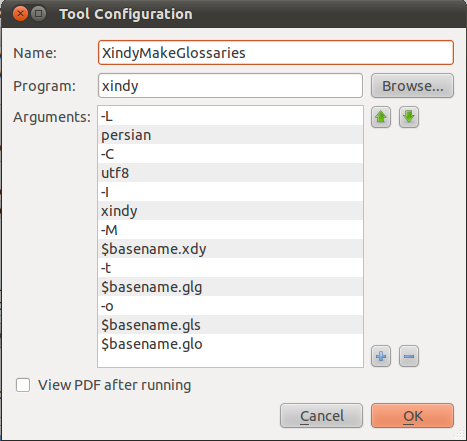
\includegraphics[width=0.7\textwidth]{Xindy_Make_Glossaries.png}}
\end{figure}
\پایان{فقرات}
\فقره 
یک بار دیگر \XeLaTeX را روی فایل خود اجرا کنید.
\پایان{شمارش}


\gls{گروه} \gls{چنبره} \gls{پردازشگر}
\gls{کلاف} \gls{شما}\gls{رایانه}\gls{واژه‌نامه}
\gls{زی‌پرشین}\gls{موسیقی} \gls{شعر}\gls{آنتن}

%%%%%%%%%%%%%%%%%%%%%%%%%%%%%
\قسمت*{نوع \lr{mylist}}
\glossarystyle{mylist}
\printglossaries
%%%%%%%%%%%%%%%%%%%%%%%%%%%%%
\صفحه‌جدید
\قسمت*{نوع \lr{list}}
\glossarystyle{list}
\printglossaries
%%%%%%%%%%%%%%%%%%%%%%%%%%%%%
\صفحه‌جدید
\glossarystyle{altlist}
\قسمت*{نوع \lr{altlist}}

\printglossaries
%%%%%%%%%%%%%%%%%%%%%%%%%%%%%
\صفحه‌جدید
\قسمت*{نوع \lr{index}}
\glossarystyle{index}
\printglossaries
%%%%%%%%%%%%%%%%%%%%%%%%%%%%%
\صفحه‌جدید
\قسمت*{نوع \lr{tree}}
\glossarystyle{tree}
\printglossaries

%%%%%%%%%%%%%%%%%%%%%%%%%%%%%
\صفحه‌جدید
\قسمت*{نوع \lr{super}}
\glossarystyle{super}
\printglossaries
%%%%%%%%%%%%%%%%%%%%%%%%%%%%%
\end{document}

